\documentclass[a4paper,12pt]{article}

% -----------------------------
% Пакеты для русского текста и математики
% -----------------------------
\usepackage[utf8]{inputenc}
\usepackage[T2A]{fontenc}
\usepackage[english,russian]{babel}
\usepackage{amsmath, amssymb}
\usepackage{mathtools}
\usepackage{physics}

% -----------------------------
% Оформление страницы, таблиц и рисунков
% -----------------------------
\usepackage{geometry}
\geometry{left=25mm,right=20mm,top=20mm,bottom=20mm}
\usepackage{graphicx}
\usepackage{float}
\usepackage{booktabs}
\usepackage{array}
\usepackage{longtable}
\usepackage{multirow}
\usepackage{makecell}
\usepackage{caption}
\usepackage{subcaption}
\usepackage{indentfirst}
\usepackage{enumitem}
\usepackage{titlesec}
\usepackage{tikz}
\usepackage{pgfplots}
\pgfplotsset{compat=1.18}

% -----------------------------
% Единицы измерения и ссылки
% -----------------------------
\usepackage{siunitx}
\sisetup{
    output-decimal-marker = {,},
    group-separator = {\,},
    per-mode = symbol
}
\usepackage[colorlinks=true, linkcolor=black, urlcolor=blue, citecolor=black]{hyperref}

\setlength{\parindent}{1.25cm}
\setlength{\parskip}{0.2em}
\renewcommand{\arraystretch}{1.25}
\titleformat{\section}{\normalfont\Large\bfseries}{\thesection}{1em}{}

\begin{document}

\begin{titlepage}
    \centering
    Санкт-Петербургский национальный исследовательский институт\\
    информационных технологий, механики и оптики\\[2.0cm]

    {\Large \textbf{ОТЧЁТ ПО ЛАБОРАТОРНОЙ РАБОТЕ №4.14}}\\[0.5cm]
    {\Large \textbf{``Спектрометр''}}\\[2.0cm]

    \begin{flushleft}
    Группа: Z3244\\[0.3cm]
    Студенты:\\
    Поминов Вадим\\
    Забродский Александр\\
    Фадеев Марк\\[0.5cm]
    Преподаватель:\\
    Калантаевский Иван Эдуардович\\[1.0cm]
    К работе допущен:\\[0.3cm]
    Работа выполнена:\\[0.3cm]
    Отчет принят:
    \end{flushleft}

    \vfill
    Санкт-Петербург\\
    \the\year
\end{titlepage}

\section{Цель работы}

\begin{enumerate}[label=\arabic*.]
    \item Определение длин волн спектрального источника.
    \item Определение показателя преломления стекла для различных длин волн с помощью спектрометра на основе призмы и дифракционной решетки.
\end{enumerate}

\section{Задачи}

\begin{enumerate}[label=\arabic*.]
    \item Произвести сборку и юстировку спектрометра с призмой и дифракционной решеткой.
    \item Получить спектры фотодиода и ртутной лампы.
    \item Определить длины волн спектра ртути.
    \item Определить показатель преломления призмы.
\end{enumerate}

\section{Объект исследования}

Объектом исследования является спектральное излучение источников света, проходящее через дисперсионные элементы спектрометра: дифракционную решетку и равностороннюю стеклянную призму.

\section{Метод исследования}

В работе используются прямые измерения линейных расстояний $x$ и $y$ с помощью линейки. Далее по измеренным расстояниям вычисляются углы отклонения лучей, длины волн спектральных линий ртути и показатель преломления стекла призмы. Таким образом, основные результаты являются результатами косвенных измерений.

\section{Рабочие формулы и исходные данные}

\subsection{Дифракционная решетка}

Для дифракционной решетки используется уравнение
\begin{equation}
    \sin\Theta_k = k\lambda g,
    \label{eq:grating}
\end{equation}
где $\Theta_k$ --- угол отклонения дифракционного максимума порядка $k$, $\lambda$ --- длина волны, $g$ --- плотность штрихов решетки.

В работе использовалась отражательная дифракционная решетка с плотностью
\begin{equation}
    g = 1200~\text{штр/мм}.
\end{equation}
Измерения проводились для первого порядка дифракции:
\begin{equation}
    k = 1.
\end{equation}

Угол отклонения определяется из геометрии установки:
\begin{equation}
    \Theta = \arctan\frac{y}{x},
    \label{eq:theta}
\end{equation}
где $x$ --- горизонтальное расстояние до экрана, $y$ --- смещение спектральной линии относительно нулевого порядка.

Так как
\begin{equation}
    \sin\Theta = \frac{y}{\sqrt{x^2+y^2}},
\end{equation}
то длина волны может быть найдена по формуле
\begin{equation}
    \lambda = \frac{1}{kg}\frac{y}{\sqrt{x^2+y^2}}.
    \label{eq:lambda}
\end{equation}
При расчете в нанометрах используется перевод $1~\text{мм}=10^6~\text{нм}$:
\begin{equation}
    \lambda_{\text{нм}} = \frac{10^6}{kg}\frac{y}{\sqrt{x^2+y^2}}.
    \label{eq:lambda_nm}
\end{equation}

Для желтой линии ртути в таблице используется значение
\begin{equation}
    \lambda_{\text{теор}} = 578~\text{нм},
\end{equation}
поскольку желтая область спектра ртути представляет собой близкий дублет $577/579~\text{нм}$, а для расчетов удобно брать среднее значение.

\subsection{Призма}

Для измерения показателя преломления призмы используется угол минимального отклонения $\gamma$. Он определяется по измеренным расстояниям:
\begin{equation}
    \gamma = \arctan\frac{y}{x}.
    \label{eq:gamma}
\end{equation}

Призма равносторонняя, поэтому угол при вершине
\begin{equation}
    A = 60^\circ.
\end{equation}

Выведем формулу для показателя преломления. В положении минимального отклонения ход луча в призме симметричен, поэтому
\begin{equation}
    r_1 = r_2 = \frac{A}{2},
\end{equation}
а углы падения и выхода равны:
\begin{equation}
    i_1=i_2=\frac{A+\gamma}{2}.
\end{equation}
По закону Снеллиуса для перехода из воздуха в стекло:
\begin{equation}
    \sin i = n\sin r.
\end{equation}
Отсюда показатель преломления призмы равен
\begin{equation}
    n = \frac{\sin\left(\dfrac{A+\gamma}{2}\right)}{\sin\left(\dfrac{A}{2}\right)}.
    \label{eq:n_prism}
\end{equation}

Для сравнения с теорией используется обратная формула для минимального угла отклонения:
\begin{equation}
    \gamma_{\text{теор}} = 2\arcsin\left(n_{\text{теор}}\sin\frac{A}{2}\right)-A.
    \label{eq:gamma_theor}
\end{equation}

Эталонные значения показателя преломления взяты для стекла SCHOTT F2: для линии около $436~\text{нм}$ используется $n_{\text{теор}}=1{,}64202$, для линии около $546~\text{нм}$ используется $n_{\text{теор}}=1{,}62408$.

\section{Измерительные приборы и элементы установки}

\begin{table}[H]
\centering
\caption{Измерительные приборы и элементы установки}
\begin{tabular}{|>{\raggedright\arraybackslash}p{5cm}|>{\raggedright\arraybackslash}p{5cm}|>{\raggedright\arraybackslash}p{4cm}|}
\hline
Наименование & Использование & Погрешность / характеристика \\
\hline
Линейка & Измерение расстояний $x$ и $y$ & $\Delta x=\Delta y=1~\text{мм}=0{,}1~\text{см}$ \\
\hline
Дифракционная решетка & Разложение света в спектр & $g=1200~\text{штр/мм}$ \\
\hline
Равносторонняя призма & Разложение света за счет дисперсии & $A=60^\circ$ \\
\hline
Ртутная лампа & Источник линейчатого спектра & --- \\
\hline
Белый светодиод & Наблюдение спектра светодиода & --- \\
\hline
Линзы & Формирование изображения щели & $f=50~\text{мм}$ и $f=100~\text{мм}$ \\
\hline
Экран & Наблюдение спектральных линий & --- \\
\hline
\end{tabular}
\end{table}

\section{Проведение измерений}

Сначала была собрана и отъюстирована схема спектрометра. Источник света, щель, линзы и дисперсионный элемент располагались на одной оптической оси. Сначала наблюдался спектр белого светодиода, затем светодиод был заменен на ртутную лампу.

При работе с дифракционной решеткой измерялись расстояния $x$ и $y$ для трех наиболее заметных линий ртути. Расстояние $x$ было одинаковым, так как экран не перемещался, а расстояние $y$ отличалось для разных спектральных линий.

При работе с призмой дифракционная решетка была заменена на равностороннюю призму. Для выбранных спектральных линий ртути призма поворачивалась до положения минимального отклонения. После этого измерялись расстояния $x$ и $y$, по которым определялся угол $\gamma$.

Схема установки с основными расстояниями приведена на рисунке~\ref{fig:scheme}.

\begin{figure}[H]
    \centering
    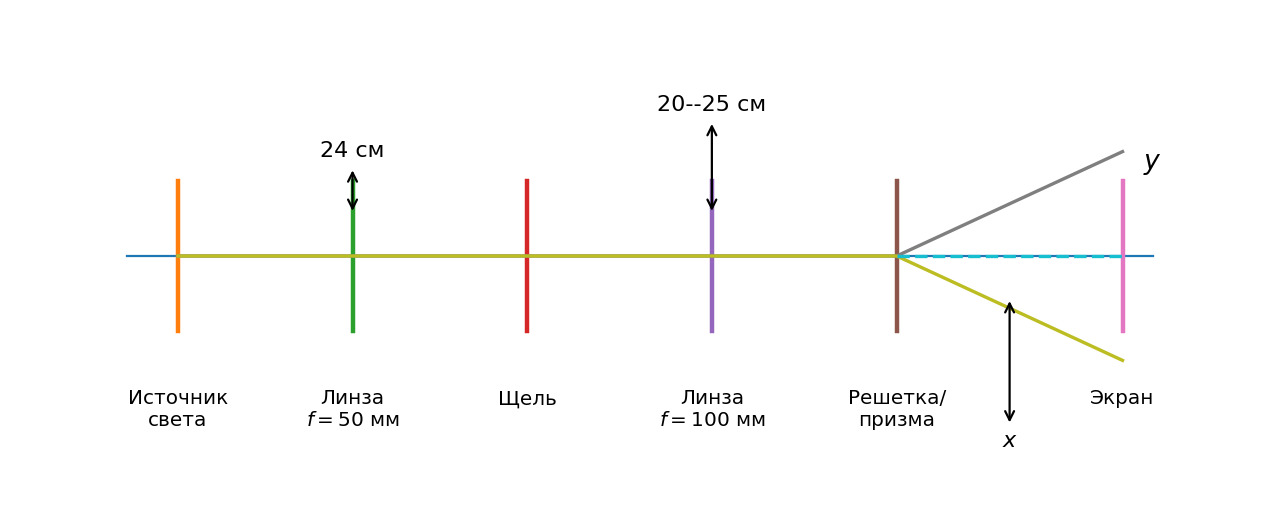
\includegraphics[width=0.95\linewidth]{figures/spectrometer_scheme.png}
    \caption{Схема спектрометра с указанием основных расстояний между элементами.}
    \label{fig:scheme}
\end{figure}

\section{Результаты прямых измерений}

\subsection{Измерения с дифракционной решеткой}

\begin{table}[H]
\centering
\caption{Измерение спектральных линий ртути с помощью дифракционной решетки}
\begin{tabular}{|c|c|c|c|c|}
\hline
№ & Линия & $x$, см & $y$, см & $\lambda_{\text{теор}}$, нм \\
\hline
1 & Фиолетовая & 25{,}0 & 15{,}2 & 436 \\
\hline
2 & Зеленая & 25{,}0 & 16{,}3 & 546 \\
\hline
3 & Желтая & 25{,}0 & 18{,}3 & 578 \\
\hline
\end{tabular}
\end{table}

\subsection{Измерения с призмой}

Так как в журнале измерений цвета линий для призмы не были отдельно зафиксированы, сопоставление с теоретическими значениями выполнено для двух характерных линий ртути: $436~\text{нм}$ и $546~\text{нм}$.

\begin{table}[H]
\centering
\caption{Измерение угла минимального отклонения призмы}
\begin{tabular}{|c|c|c|c|}
\hline
№ & Принятая линия сравнения, нм & $x$, см & $y$, см \\
\hline
1 & 436 & 17{,}0 & 27{,}0 \\
\hline
2 & 546 & 18{,}0 & 25{,}0 \\
\hline
\end{tabular}
\end{table}

\section{Обработка результатов}

\subsection{Расчет длин волн спектра ртути}

Рассчитаем угол отклонения и длину волны для первой линии:
\begin{equation}
    \Theta_1 = \arctan\frac{15{,}2}{25{,}0}=31{,}30^\circ.
\end{equation}

\begin{equation}
    \lambda_1 = \frac{\sin 31{,}30^\circ}{1\cdot 1200}~\text{мм}
    =0{,}0004329~\text{мм}=432{,}9~\text{нм}.
\end{equation}

Для второй линии:
\begin{equation}
    \Theta_2 = \arctan\frac{16{,}3}{25{,}0}=33{,}10^\circ,
\end{equation}
\begin{equation}
    \lambda_2 = \frac{\sin 33{,}10^\circ}{1200}~\text{мм}
    =0{,}0004551~\text{мм}=455{,}1~\text{нм}.
\end{equation}

Для третьей линии:
\begin{equation}
    \Theta_3 = \arctan\frac{18{,}3}{25{,}0}=36{,}20^\circ,
\end{equation}
\begin{equation}
    \lambda_3 = \frac{\sin 36{,}20^\circ}{1200}~\text{мм}
    =0{,}0004922~\text{мм}=492{,}2~\text{нм}.
\end{equation}

Итоговые результаты для решетки представлены в таблице~\ref{tab:grating_results}.

\begin{table}[H]
\centering
\caption{Расчет экспериментальных длин волн}
\label{tab:grating_results}
\begin{tabular}{|c|c|c|c|c|c|}
\hline
№ & Линия & $\Theta$, $^\circ$ & $\lambda_{\text{эксп}}$, нм & $\lambda_{\text{теор}}$, нм & $\varepsilon$, \% \\
\hline
1 & Фиолетовая & 31{,}30 & $432{,}9\pm2{,}4$ & 436 & 0{,}7 \\
\hline
2 & Зеленая & 33{,}10 & $455{,}1\pm2{,}3$ & 546 & 16{,}6 \\
\hline
3 & Желтая & 36{,}20 & $492{,}2\pm2{,}2$ & 578 & 14{,}8 \\
\hline
\end{tabular}
\end{table}

\subsection{Погрешность длин волн}

Погрешность прямых измерений принимаем равной цене деления линейки:
\begin{equation}
    \Delta x=\Delta y=0{,}1~\text{см}.
\end{equation}

Запишем формулу для длины волны в виде
\begin{equation}
    \lambda = C\frac{y}{\sqrt{x^2+y^2}}, \qquad C=\frac{10^6}{kg}.
\end{equation}

Тогда частные производные равны
\begin{equation}
    \pdv{\lambda}{x}=-C\frac{xy}{(x^2+y^2)^{3/2}},
\end{equation}
\begin{equation}
    \pdv{\lambda}{y}=C\frac{x^2}{(x^2+y^2)^{3/2}}.
\end{equation}

Погрешность длины волны определяется по формуле
\begin{equation}
    \Delta\lambda=\sqrt{\left(\pdv{\lambda}{x}\Delta x\right)^2+\left(\pdv{\lambda}{y}\Delta y\right)^2}.
\end{equation}

Для первой линии получаем
\begin{equation}
    \Delta\lambda_1\approx2{,}4~\text{нм}.
\end{equation}
Для второй и третьей линий аналогично:
\begin{equation}
    \Delta\lambda_2\approx2{,}3~\text{нм}, \qquad
    \Delta\lambda_3\approx2{,}2~\text{нм}.
\end{equation}

Относительное расхождение с табличным значением вычислялось по формуле
\begin{equation}
    \varepsilon = \frac{|\lambda_{\text{эксп}}-\lambda_{\text{теор}}|}{\lambda_{\text{теор}}}\cdot100\%.
\end{equation}

\subsection{Расчет показателя преломления призмы}

Для первой строки таблицы измерений:
\begin{equation}
    \gamma_1=\arctan\frac{27{,}0}{17{,}0}=57{,}80^\circ.
\end{equation}

Тогда
\begin{equation}
    n_1=\frac{\sin\left(\dfrac{60^\circ+57{,}80^\circ}{2}\right)}{\sin30^\circ}=1{,}713.
\end{equation}

Для второй строки:
\begin{equation}
    \gamma_2=\arctan\frac{25{,}0}{18{,}0}=54{,}25^\circ,
\end{equation}
\begin{equation}
    n_2=\frac{\sin\left(\dfrac{60^\circ+54{,}25^\circ}{2}\right)}{\sin30^\circ}=1{,}680.
\end{equation}

Теоретический угол минимального отклонения для стекла F2 находился по формуле~\eqref{eq:gamma_theor}. Для линии $436~\text{нм}$:
\begin{equation}
    \gamma_{\text{теор},1}=2\arcsin\left(1{,}64202\cdot \sin30^\circ\right)-60^\circ=50{,}37^\circ.
\end{equation}
Для линии $546~\text{нм}$:
\begin{equation}
    \gamma_{\text{теор},2}=2\arcsin\left(1{,}62408\cdot \sin30^\circ\right)-60^\circ=48{,}59^\circ.
\end{equation}

Результаты представлены в таблице~\ref{tab:prism_results}.

\begin{table}[H]
\centering
\caption{Определение показателя преломления стекла призмы}
\label{tab:prism_results}
\begin{tabular}{|c|c|c|c|c|c|c|c|}
\hline
№ & $\lambda$, нм & $x$, см & $y$, см & $\gamma_{\text{эксп}}$, $^\circ$ & $\gamma_{\text{теор}}$, $^\circ$ & $n_{\text{эксп}}$ & $n_{\text{теор}}$ \\
\hline
1 & 436 & 17{,}0 & 27{,}0 & $57{,}80\pm0{,}18$ & 50{,}37 & $1{,}713\pm0{,}002$ & 1{,}64202 \\
\hline
2 & 546 & 18{,}0 & 25{,}0 & $54{,}25\pm0{,}19$ & 48{,}59 & $1{,}680\pm0{,}002$ & 1{,}62408 \\
\hline
\end{tabular}
\end{table}

\subsection{Погрешность показателя преломления}

Для угла
\begin{equation}
    \gamma=\arctan\frac{y}{x}
\end{equation}
частные производные равны
\begin{equation}
    \pdv{\gamma}{x}= -\frac{y}{x^2+y^2}, \qquad
    \pdv{\gamma}{y}= \frac{x}{x^2+y^2}.
\end{equation}

Следовательно,
\begin{equation}
    \Delta\gamma = \sqrt{\left(\pdv{\gamma}{x}\Delta x\right)^2+
    \left(\pdv{\gamma}{y}\Delta y\right)^2}.
\end{equation}

Для показателя преломления
\begin{equation}
    n = \frac{\sin\left(\dfrac{A+\gamma}{2}\right)}{\sin\left(\dfrac{A}{2}\right)}
\end{equation}
производная по $\gamma$ равна
\begin{equation}
    \pdv{n}{\gamma}=\frac{1}{2}\frac{\cos\left(\dfrac{A+\gamma}{2}\right)}{\sin\left(\dfrac{A}{2}\right)}.
\end{equation}

Тогда
\begin{equation}
    \Delta n = \left|\pdv{n}{\gamma}\right|\Delta\gamma.
\end{equation}

После подстановки чисел получаем:
\begin{equation}
    \Delta n_1 \approx 0{,}002, \qquad \Delta n_2 \approx 0{,}002.
\end{equation}

Относительное расхождение с табличным показателем преломления:
\begin{equation}
    \varepsilon_n = \frac{|n_{\text{эксп}}-n_{\text{теор}}|}{n_{\text{теор}}}\cdot100\%.
\end{equation}

Для первой строки:
\begin{equation}
    \varepsilon_{n1}=\frac{|1{,}713-1{,}64202|}{1{,}64202}\cdot100\%\approx4{,}3\%.
\end{equation}

Для второй строки:
\begin{equation}
    \varepsilon_{n2}=\frac{|1{,}680-1{,}62408|}{1{,}62408}\cdot100\%\approx3{,}4\%.
\end{equation}

\section{Графики}

На рисунке~\ref{fig:wavelength_comparison} показано сравнение экспериментальных длин волн, полученных с помощью дифракционной решетки, с табличными значениями.

\begin{figure}[H]
    \centering
    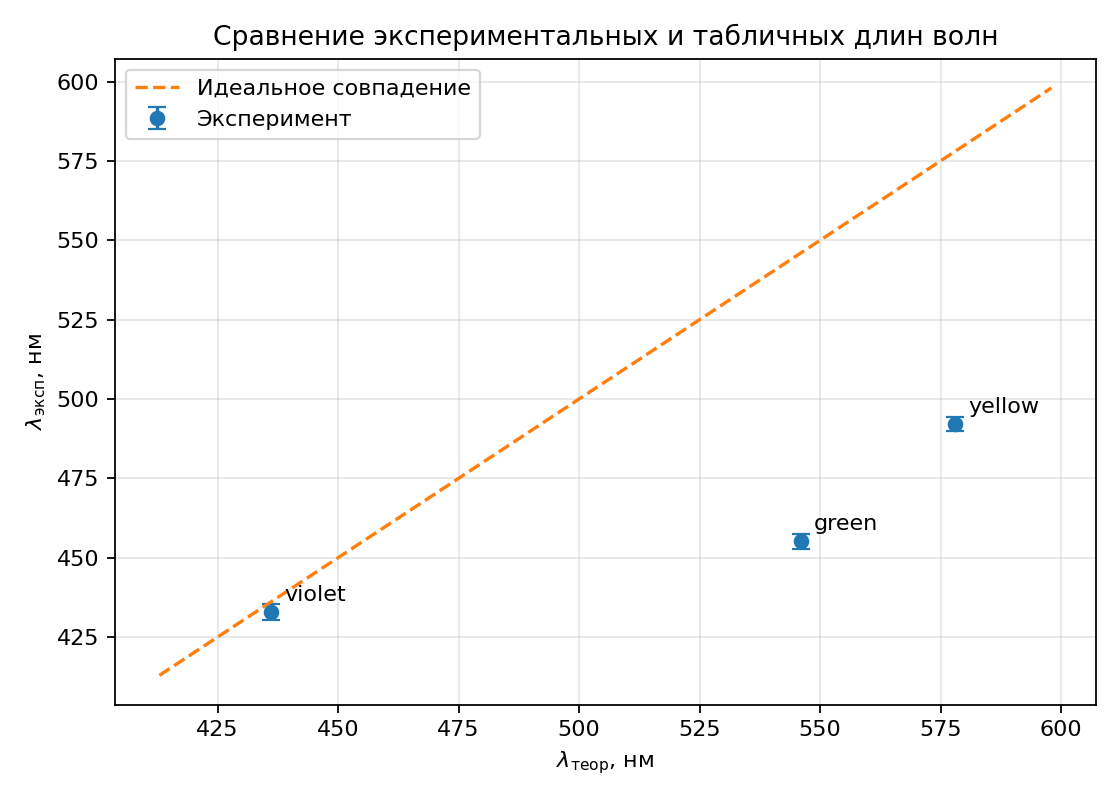
\includegraphics[width=0.85\linewidth]{figures/wavelength_comparison.png}
    \caption{Сравнение экспериментальных и табличных длин волн спектральных линий ртути.}
    \label{fig:wavelength_comparison}
\end{figure}

На рисунке~\ref{fig:prism_n} показано сравнение экспериментального показателя преломления призмы с табличными значениями для стекла F2.

\begin{figure}[H]
    \centering
    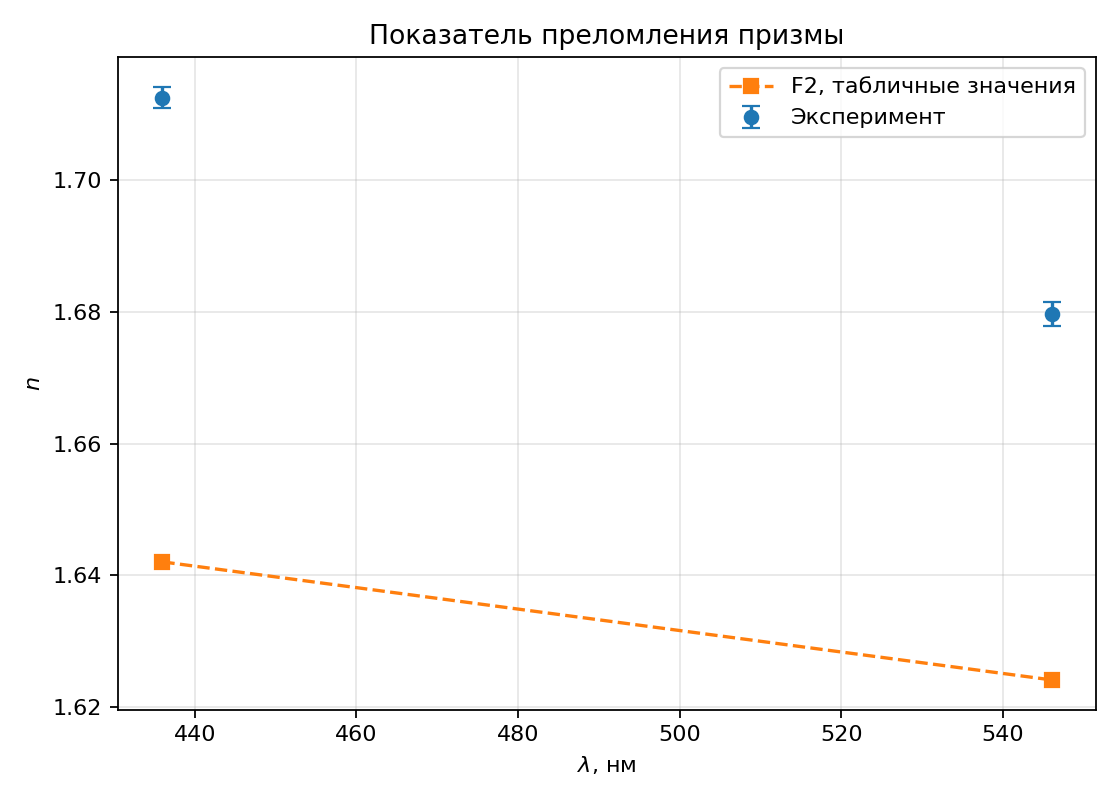
\includegraphics[width=0.85\linewidth]{figures/prism_refractive_index.png}
    \caption{Показатель преломления призмы: эксперимент и табличные значения F2.}
    \label{fig:prism_n}
\end{figure}

\section{Окончательные результаты}

\begin{enumerate}[label=\arabic*.]
    \item Для фиолетовой линии ртути получено:
    \begin{equation}
        \lambda_1=(432{,}9\pm2{,}4)~\text{нм}.
    \end{equation}
    Табличное значение: $436~\text{нм}$. Расхождение составляет около $0{,}7\%$.

    \item Для зеленой линии ртути получено:
    \begin{equation}
        \lambda_2=(455{,}1\pm2{,}3)~\text{нм}.
    \end{equation}
    Табличное значение: $546~\text{нм}$. Расхождение составляет около $16{,}6\%$.

    \item Для желтой линии ртути получено:
    \begin{equation}
        \lambda_3=(492{,}2\pm2{,}2)~\text{нм}.
    \end{equation}
    Для сравнения использовалось среднее табличное значение желтого дублета $578~\text{нм}$. Расхождение составляет около $14{,}8\%$.

    \item Для призмы получены значения показателя преломления:
    \begin{equation}
        n_1 = 1{,}713\pm0{,}002,
    \end{equation}
    \begin{equation}
        n_2 = 1{,}680\pm0{,}002.
    \end{equation}
    Табличные значения для стекла F2: $1{,}64202$ и $1{,}62408$ соответственно. Относительные расхождения составляют около $4{,}3\%$ и $3{,}4\%$.
\end{enumerate}

\section{Выводы и анализ результатов работы}

В ходе лабораторной работы была собрана и отъюстирована установка спектрометра. Были получены спектры белого светодиода и ртутной лампы. Для ртутной лампы были измерены положения трех спектральных линий при использовании дифракционной решетки, после чего по уравнению решетки были рассчитаны экспериментальные длины волн.

Наиболее точный результат получен для фиолетовой линии: $\lambda=(432{,}9\pm2{,}4)~\text{нм}$ при табличном значении $436~\text{нм}$. Расхождение составляет около $0{,}7\%$, что является хорошим результатом для измерения линейкой.

Для зеленой и желтой линий получены значения, заметно отличающиеся от табличных. Возможные причины расхождения: неточное определение положения нулевого порядка, ошибка измерения смещения $y$, неидеальная юстировка решетки, неперпендикулярность экрана, а также возможная ошибка идентификации спектральных линий.

Также была получена формула связи минимального угла отклонения луча в равносторонней призме с показателем преломления. По результатам измерений получены значения $n_1=1{,}713\pm0{,}002$ и $n_2=1{,}680\pm0{,}002$. Они больше табличных значений для стекла F2. Это может быть связано с тем, что призма была установлена не точно в положении минимального отклонения, а также с трудностью выбора точки отсчета внутри призмы и на экране.

Таким образом, качественно работа спектрометра была подтверждена: разные длины волн отклоняются на разные расстояния, а показатель преломления зависит от длины волны. При этом количественная точность результатов существенно зависит от аккуратности юстировки и измерения геометрических расстояний.

\begin{thebibliography}{9}
\bibitem{lab414}
Методическое описание лабораторной работы №4.14 ``Спектрометр'', физический факультет ФТМФ ИТМО.

\bibitem{schottf2}
SCHOTT Advanced Optics. Optical glass F2: refractive index data for spectral lines.
\end{thebibliography}

\end{document}
